
%%%%%%%%%%%%%%%%%%%%%%%%%%%%%%%%%%%%%%%%%%%%%%%%%%%%%%%%%%%%%%%%%%%%%%%%%%%%%%%%
%2345678901234567890123456789012345678901234567890123456789012345678901234567890
%        1         2         3         4         5         6         7         8
% \documentclass[letterpaper, 10 pt, conference]{ieeeconf}  % Comment this line out
                                                          % if you need a4paper
\documentclass[a4paper, 10pt, conference]{ieeeconf}      % Use this line for a4
\synctex=1                                                          % paper

\IEEEoverridecommandlockouts                              % This command is only
                                                          % needed if you want to
                                                          % use the \thanks command
\overrideIEEEmargins
% See the \addtolength command later in the file to balance the column lengths
% on the last page of the document


% The following packages can be found on http:\\www.ctan.org
\usepackage{graphicx} % for pdf, bitmapped graphics files
%\usepackage{epsfig} % for postscript graphics files
%\usepackage{mathptmx} % assumes new font selection scheme installed
\usepackage{times} % assumes new font selection scheme installed
\usepackage{amsmath} % assumes amsmath package installed
\usepackage{amssymb}  % assumes amsmath package installed
\usepackage{verbatim} % for comment
\usepackage{cite}
\usepackage{subfigure}
\usepackage[hyphens]{url}
\usepackage{float}
\usepackage{tabulary}
\usepackage{tabularx}
\usepackage{lipsum,amsmath,multicol}
\usepackage{tensor}
\usepackage{multirow}
\usepackage{booktabs}
\usepackage{flafter}
%\usepackage{todonotes}
\usepackage[disable]{todonotes}
\usepackage[nolist]{acronym}
%\usepackage[]{natbib}
\usepackage{tikz}
%\usepackage[outdir=./fig/]{epstopdf}
%\graphicspath
    
\usepackage{lipsum}
\usepackage{siunitx}
\usepackage[capitalise]{cleveref}
\usepackage{booktabs}
%\usepackage{subcaption}
\pdfminorversion=4
\pdfobjcompresslevel=2


\RequirePackage{algorithmicx}
% \RequirePackage{algorithmic}
\usepackage[noend]{algpseudocode}
\RequirePackage{algorithm}
\newcommand*\Let[2]{\State #1 $\gets$ #2}

\renewcommand{\vec}[1]{\mathbf{#1}}
%\usepackage[lmargin=19.1mm,rmargin=19.1mm,tmargin=25.4mm,bmargin=19.1mm]{geometry}
%\usepackage[top=36.7mm,left=19.1mm,right=13.1mm,bottom=19.1mm]{geometry}
%\usepackage{hyperref}

\usepackage{color}

\def\TODO#1{{\color{red}{\bf [TODO:} {\it{#1}}{\bf ]}}} \def\OUTLINE#1{{\color{green}{\bf [Outline:} {\it{#1}}{\bf ]}}}
\def\NOTE#1{{\bf [NOTE:} {\it\color{blue}{#1}}{\bf ]}.} \def\CHK#1{{\bf [CHECK:} {\it\color{red} {#1}}{\bf ]}.}

\DeclareMathOperator{\atantwo}{atan2}
\DeclareMathOperator*{\argmaxOp}{argmax}
\newcommand*{\argmax}{\argmaxOp\limits}

\newcommand\encircle[1]{%
  \tikz[baseline=(X.base)] 
    \node (X) [draw, shape=circle, inner sep=0] {\strut #1};}

\makeatletter
\newenvironment{myalign*}{%
  \setlength{\mathindent}{0pt}%
  \setlength{\abovedisplayskip}{-\baselineskip}%
  \setlength{\abovedisplayshortskip}{\abovedisplayskip}%
  \start@align\@ne\st@rredtrue\m@ne
}%
{\endalign}
\makeatother

\title{\LARGE \bf\vspace{-4ex}
    \begin{flushleft}
  \begin{minipage}{0.7\linewidth}
      Cardiff Racing Driverless Design Progress Report: Cone Detection, Route
      Planning, and Simulation
    \end{minipage}
    \hfill
  \begin{minipage}{0.16\linewidth}
    \protect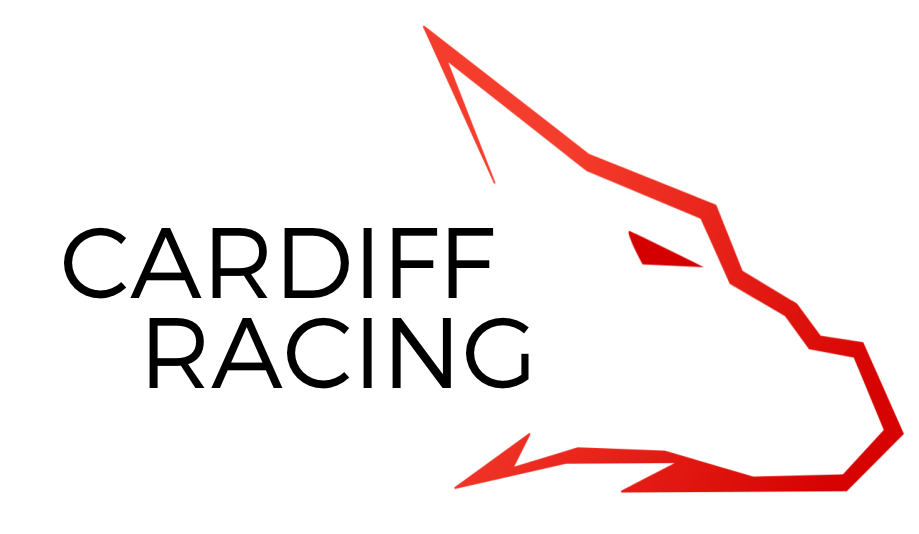
\includegraphics[width=1.0\linewidth]{cr}
  \end{minipage}
    \end{flushleft}
}


\author{
    \footnotesize Daniel Harbourne, Mohamed Binesmael, Molly Ragonnet, Matteo de Rosa, Rachael Joyce,
    Deeon Roy, Ahmad Amer, Bryson Kwan, Kirill Sidorov
}
\makeatletter
\def\bstctlcite{\@ifnextchar[{\@bstctlcite}{\@bstctlcite[@auxout]}}
\def\@bstctlcite[#1]#2{\@bsphack
  \@for\@citeb:=#2\do{%
    \edef\@citeb{\expandafter\@firstofone\@citeb}%
    \if@filesw\immediate\write\csname #1\endcsname{\string\citation{\@citeb}}\fi}%
  \@esphack}
\makeatother

\begin{document}
\bstctlcite{IEEEexample:BSTcontrol}

\maketitle

\thispagestyle{plain}
\pagestyle{plain}



%%%%%%%%%%%%%%%%%%%%
% 	Abstract
%%%%%%%%%%%%%%%%%%%%

\begin{abstract}
Formula Student UK, the Europe's most established educational engineering
competition, in which Cardiff Racing team have earned 1st place in 2017,
have recently announced the indroduction of driverless racing
discipline as part of the competition. 
This paper reports on the current progress of the Cardiff Racing Driverless
team, and discusses the software framework, the situational awareness, and the
path planning components of our system.
\end{abstract}

\section{Introduction}
Recently, autonomous (driverless) vehicle control has attracted substantial
attention in both the academia and the industry. Driverless racing is a
recently introduced discipline within the Formula Student competition.  While
driverless control in urban environments in now an established
research field, competitive driverless racing presents a number of unique
challenges and is a relatively unexplored area.  Recent advances in driverless
racing include the 2017 winner, ETH Zurich's \emph{fl\"{u}ela}~\cite{valls18},
TUW-Racing Edge8~\cite{zeilinger17}, and Beijing Institute of Technology
vehicle~\cite{ni17}, ``Junior'' in the DARPA Urban
Challenge~\cite{montemerlo08}.

\begin{figure}[t]
  \centering
  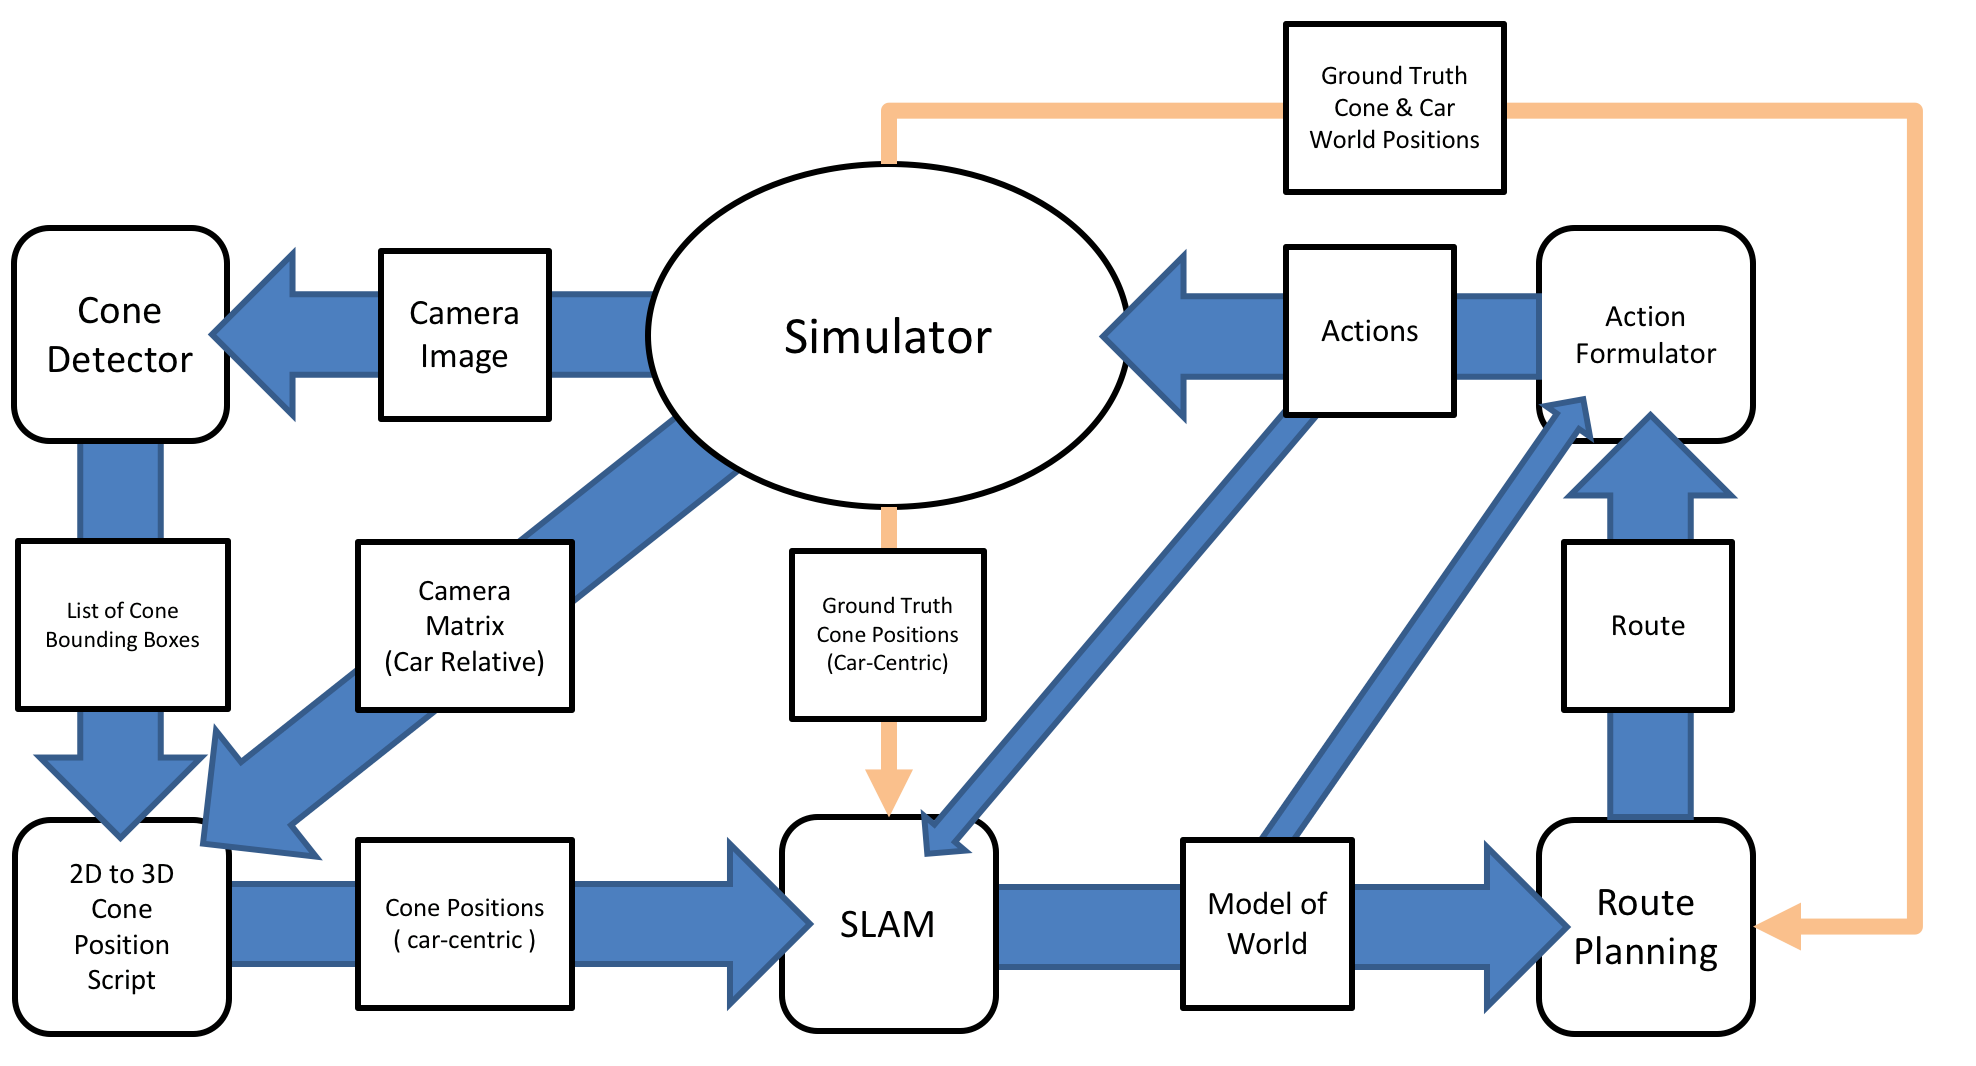
\includegraphics[width=0.95\linewidth]{img/system_new}
  \caption{System overview.}
  \label{fig:system}\vspace{-4ex}
\end{figure}
This paper reports on the current progress of the Cardiff Racing Driverless
team addressing this challenge. We have adopted a modular system architecture
with a simulator in the loop, whose overview is shown in~\cref{fig:system}. In
this paper, we address the cone detection, path planning, and simulation
components of the system.
\section{Cone Detection}
We have implemented and evaluated several approaches for cone detection and
position estimation.

First approach is the Viola-Jones cascade detector~\cite{viola01} which
consists of several stages of cheap classifiers. A sliding
window is passed through an image, and it is classified by a stage as negative
(doesn't contain the object) or positive (contains the object). If a window is
classified as negative, it is rejected and the window slides to the next
location. If it is classified as positive, the window is passed to the next
stage. The detector output a positive detection if the window is classified
positive by the final stage. Early rejection in the cascade lends to very fast
operation. We have experimented with three types of features: Haar features,
histograms of oriented gradients (HoG), and local binary patterns (LBP).

The second approach is the region-proposal CNN (RCNN)~\cite{girshick13} which
works by using a traditional computer vision technique called selective search
to identify regions of interest (ROIs), then applying a convolutional neural
network to each ROI to classify the image contained within that region. A
typical image will contain about 2000 ROIs, which each need to be classified,
making this process time-consuming.

Finally, the Fast R-CNN technique~\cite{girshick15} is similar to the R-CNN technique in that a CNN is used for classification of regions and for bounding box regression. However, unlike in R-CNNs, in Fast R-CNNs the image is passed through the CNN once, creating one large feature map. Regions of interest are then selected from this feature map and each one is passed through layers which then output bounding boxes. The main benefit is that it offers an end-to-end approach which allows for training to take place across the entire network and the forward pass time is faster. 

We have manually annotated 1088 images (988 in the training set, and 100 in
testing), containing 3106 exemplars of cones (2395 in the training set, 711 in testing).
A further 3219 negative images, including of race tracks, were used for
training of the cascade detector.

% \begin{table}
%   \hfill\begin{tabular}{lll}
%     \toprule
%     &Images&Cones\\
%     \midrule
%     Training set & 988 & 2395\\
%     Testing set& 100 & 711\\
%     Total & 1088 & 3106\\
%     \bottomrule
%   \end{tabular}\hfill
%   \caption{Cone dataset statistics.}
%   \label{tab:dataset}
% \end{table}

\begin{table}
  \centering
  \vspace{-4ex}
  \caption{Comparison of the cone detection techniques. {\Large$\tau$} is the
    intersection over union
    acceptance threshold between the detected and the ground truth bounding boxes.}
  \begin{tabular}{llrrrr}
    \toprule
    Technique&{\Large$\tau$}&Time, s/im&Precision&Recall&Avg. Prec.\\
             \midrule
    Haar& 0.5&0.099&0.6297&0.6825&0.4493\\
    Haar& 0.3& &0.7901 &0.8564 &0.7287\\
    HOG& 0.5&0.165 &0.5122& 0.6217& 0.3781\\
    HOG& 0.3& & 0.8625 & 0.7581 & 0.5724\\
    LBP& 0.5&0.092 &0.5235 &0.6259 &0.3512\\
    LBP& 0.5& &0.6882 &0.8228 &0.6393\\
    RCNN& 0.5&4.442 &0.6777 &0.3727 &0.3052\\
    RCNN& 0.3& &0.8286 &0.4557 &0.4413\\
    Fast-RCNN& 0.5&0.703 &0.2742 &0.1674 &0.0507\\
    Fast-RCNN& 0.3& &0.5968& & 0.2583\\
    \bottomrule
  \end{tabular}
  \label{tab:cone}
\end{table}
Our evaluation (see~Table~\ref{tab:cone}) shows that in this scenario the traditional computer vision
techniques perform better. We hypothesise that this is due to the regular shape of
the cones, which lends itself well to the feature detection techniques, as
well as the relatively small number of examples.

\begin{figure}
  \centering
  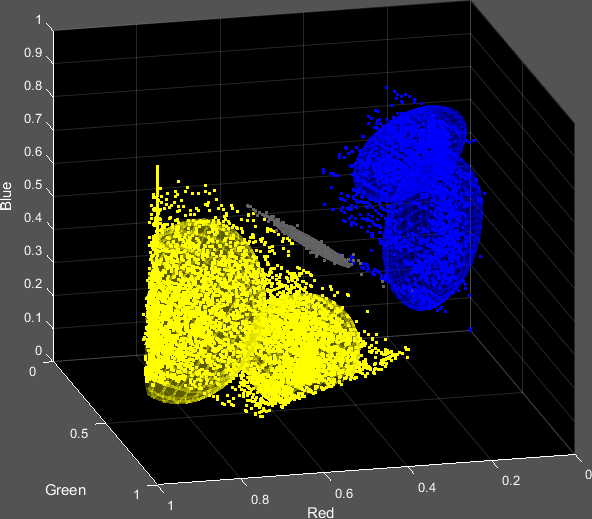
\includegraphics[width=0.43\linewidth]{img/colour_model_amz_rgb_3d}
  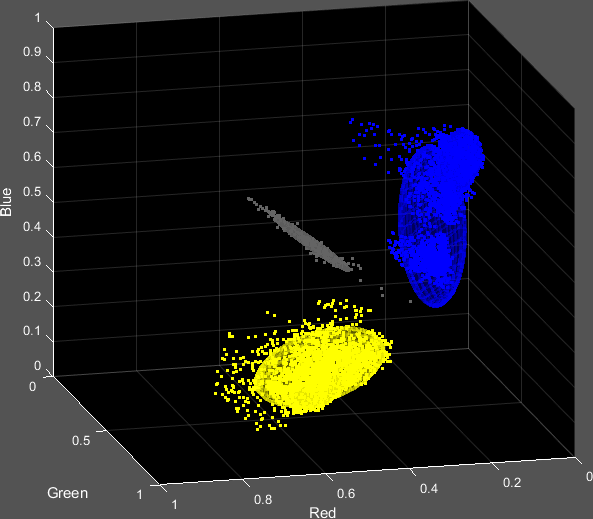
\includegraphics[width=0.43\linewidth]{img/colour_model_single_lap_rgb_3d}
  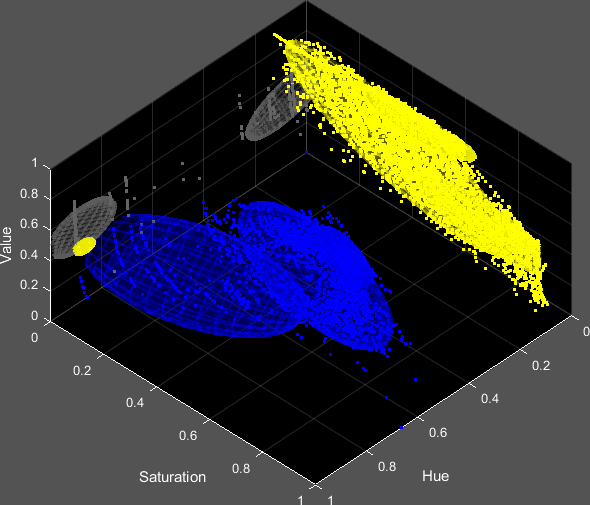
\includegraphics[width=0.43\linewidth]{img/colour_model_amz_hsv_3d}
  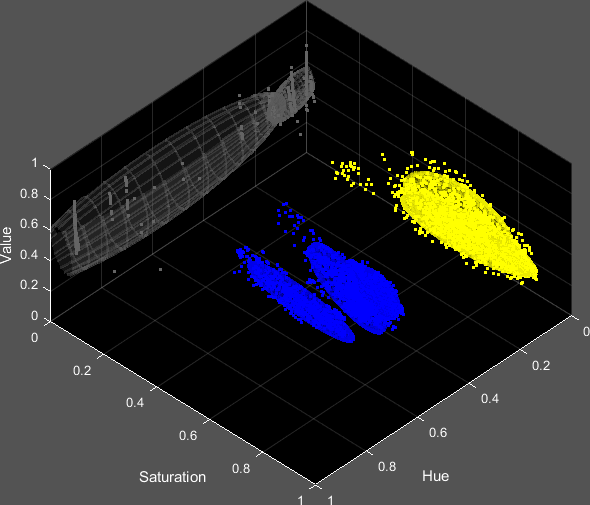
\includegraphics[width=0.43\linewidth]{img/colour_model_single_lap_hsv_3d}
  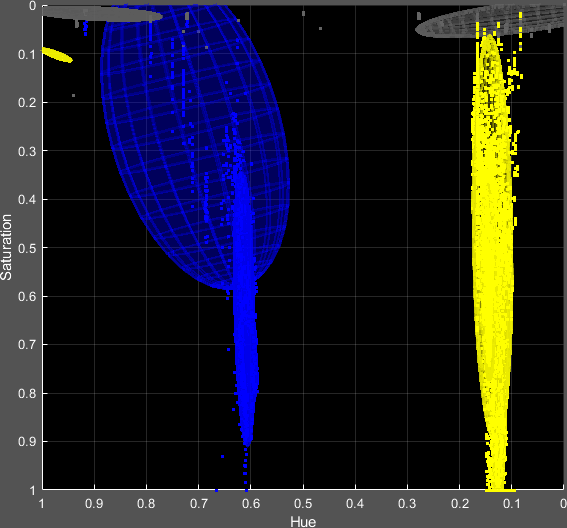
\includegraphics[width=0.43\linewidth]{img/colour_model_amz_hsv_2d}
  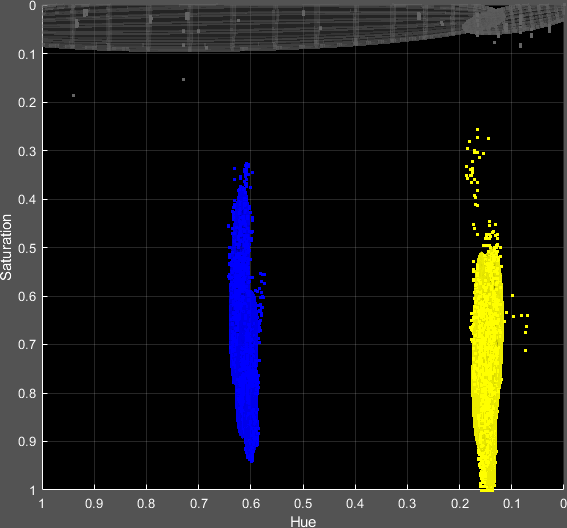
\includegraphics[width=0.43\linewidth]{img/colour_model_single_lap_hsv_2d}\\
  \qquad AMZ data\qquad\qquad\qquad StreetDrone data\hfill
  \caption{Colour model. Ellipsoids delineate one standard deviation of the
    Gaussians in the mixture. \textsl{Top:} RGB space; \textsl{Middle and
      bottom:} HSV space.}
  \label{fig:colour}
\end{figure}
Cone detection with cascade detector is done on grayscale values only.  We
further employ a statistical colour model which serves two purposes: to
differentiate blue cones from yellow ones and to further filter false positive
detections.  For this we model the distribution of cone pixel colours as a
Gaussian mixture model (GMM) which has the
form~\cite{duda00}
\begin{equation}
  p(\vec{x}) = \sum_{i=1}^n \alpha_i G(\vec{x}, \vec{\mu}_i, \vec{C}_i),
  \label{eq:gmm}
\end{equation}
where $n$ is the number of Gaussians in the mixture, $\vec{\mu}$ are the
centres of the Gaussians, $\vec{C}_i$ are the corresponding covariance
matrices, and $\alpha_i$ are the prior probabilities. The parameters of the
GMM are estimated using the well-known EM algorithm~\cite{duda00,press07}.
GMM gives a degree of invariance to changes in colour of the cones. Working in
HSV colour space gives a further degree of invariance to global illumination.
The colour models may need to be adjusted for a specific
camera. \Cref{fig:colour} show examples of GMM colour models in RGB and HSV
colour spaces.

  \begin{algorithm}[t]
    \footnotesize
    \caption{Filtering false-positives with colour model
      \label{alg:filter}}
    \begin{algorithmic}[1]
      \Require{Bounding box $W$, mixture models
        $(\vec{\mu}^b, \vec{C}^b)$,
    $(\vec{\mu^y}, \vec{C}^y)$ with $N_b$ and $N_y$ components, thresholds
$\tau_b$, $\tau_y$, $\rho_b$, $\rho_y$.}
      \State{$D^b\gets 0$, $D^y\gets 0$}
\For{\textrm{each
          pixel }$(r, g, b)\in W$}
      \Let{$\vec{x}=(h, s, v)$}{\Call{rgb2hsv}{$(r, g, b)$}}
      \State{$d^b_\mathrm{min}\gets\inf$, $d^y_\mathrm{min}\gets\inf$}
      \For{$i \gets 1 \textrm{ to } N_b$}
      \Let{$d$}{$\sqrt{(\vec{x}-\vec{\mu^b_i})(\vec{C_i}^b)^{-1}(\vec{x} -
          \vec{\mu^b_i})'}$}\Comment{Mahalanobis}
      \Let{$d^b_\mathrm{min}$}{$\min(d^b_\mathrm{min}, d)$}\Comment{min over components}
      \EndFor
      \For{$i \gets 1 \textrm{ to } N_y$}\Comment{Same for yellow}
      \Let{$d$}{$\sqrt{(\vec{x}-\vec{\mu^y_i})(\vec{C_i}^y)^{-1}(\vec{x} -
          \vec{\mu^y_i})'}$}
      \Let{$d^y_\mathrm{min}$}{$\min(d^y_\mathrm{min}, d)$}
      \EndFor
      \State{\textbf{if }$d^b_\mathrm{min} > \tau_b$\textbf{ then }$D^b\gets
        D^b+1$}\Comment{Count outliers}
      \State{\textbf{if }$d^y_\mathrm{min} > \tau_y$\textbf{ then }$D^y\gets D^y+1$}
      \If{$D^b/|W|<\rho_b$ \textbf{and} $D^y/|W|<\rho_y$}
      \State{\textbf{if }$D^b>D^y$\textbf{ then return }\texttt{FALSE\_POS\_BLUE}}
      \State{\textbf{else return }\texttt{FALSE\_POS\_YELLOW}}
      \Else
      \State{\textbf{if }$D^b>D^y$\textbf{ then return }\texttt{TRUE\_POS\_BLUE}}
      \State{\textbf{else return }\texttt{TRUE\_POS\_YELLOW}}
      \EndIf
      \EndFor
    \end{algorithmic}
  \end{algorithm}
\begin{figure}
  \centering
  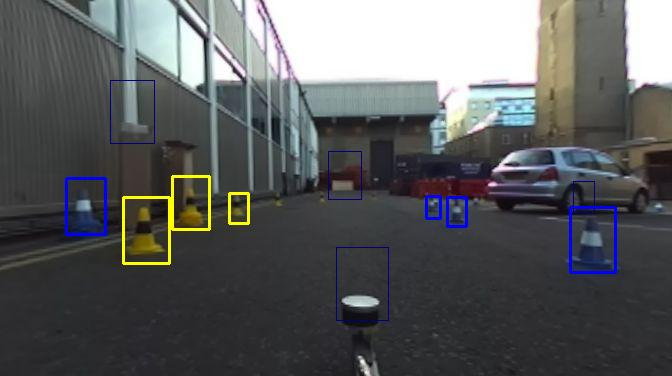
\includegraphics[width=0.45\linewidth]{img/single_lap/frame0134}
  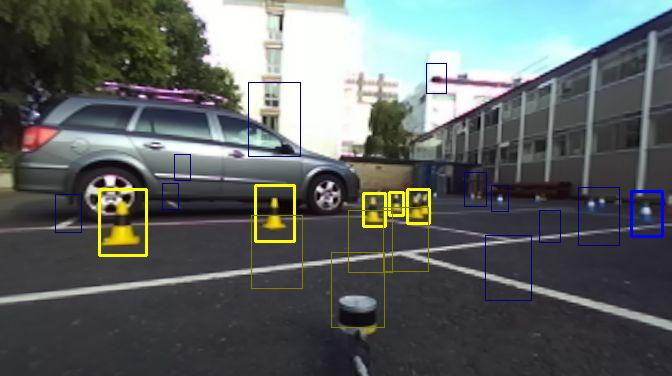
\includegraphics[width=0.45\linewidth]{img/single_lap/frame0212}
  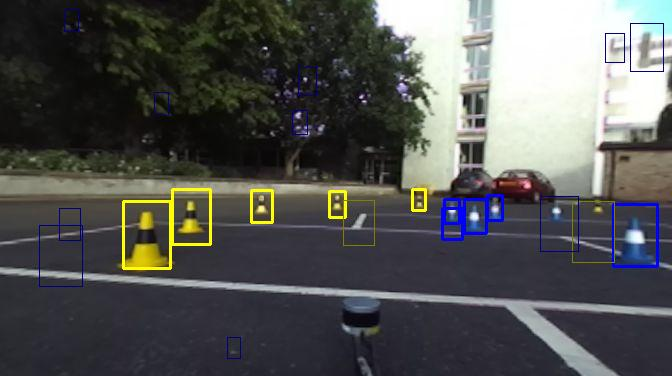
\includegraphics[width=0.45\linewidth]{img/single_lap/frame0253}
  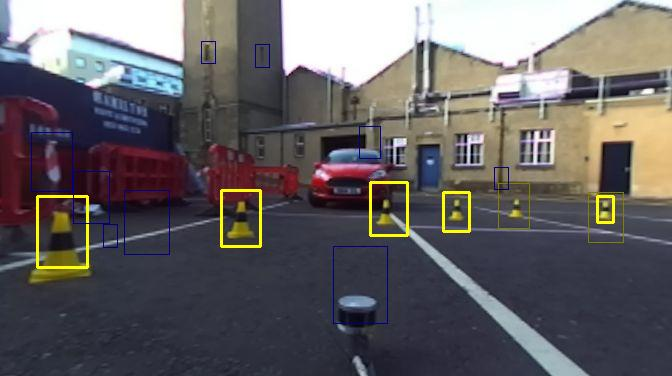
\includegraphics[width=0.45\linewidth]{img/single_lap/frame0175}
  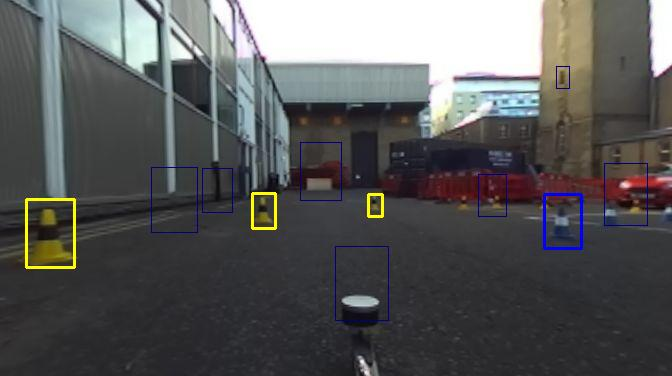
\includegraphics[width=0.45\linewidth]{img/single_lap/frame0152}
  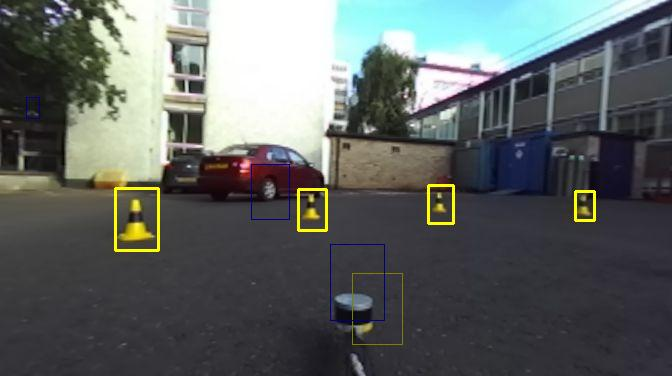
\includegraphics[width=0.45\linewidth]{img/single_lap/frame0278}\\[0.5ex]
  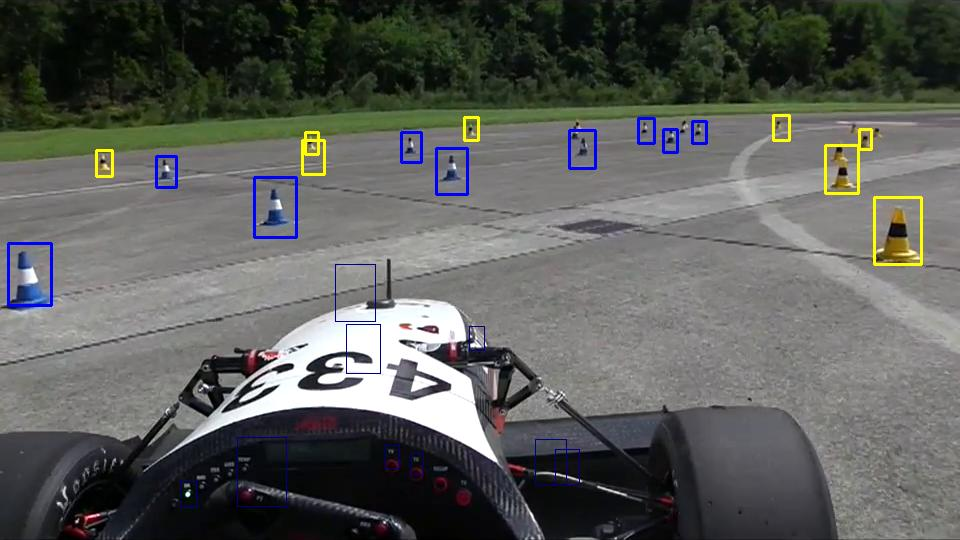
\includegraphics[width=0.45\linewidth]{img/amz/000513}
  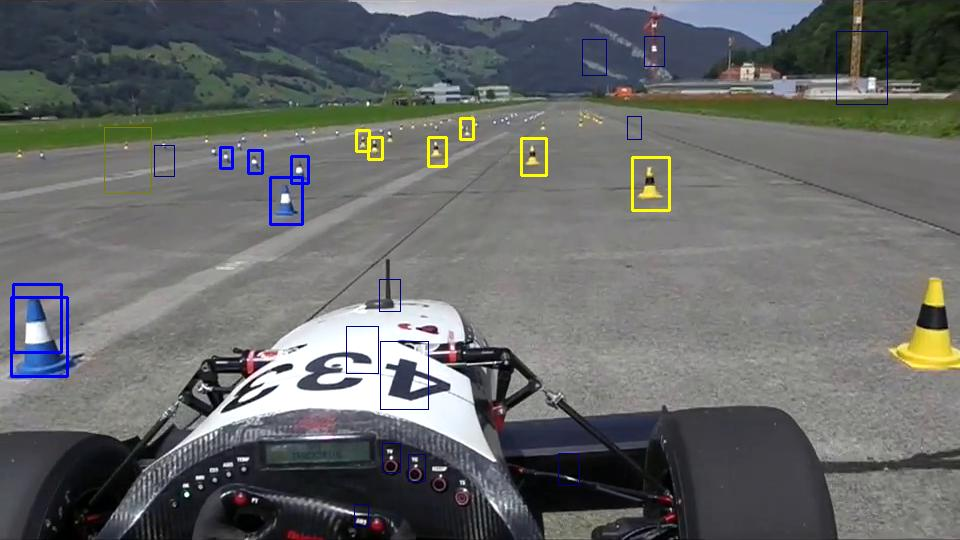
\includegraphics[width=0.45\linewidth]{img/amz/001345}
  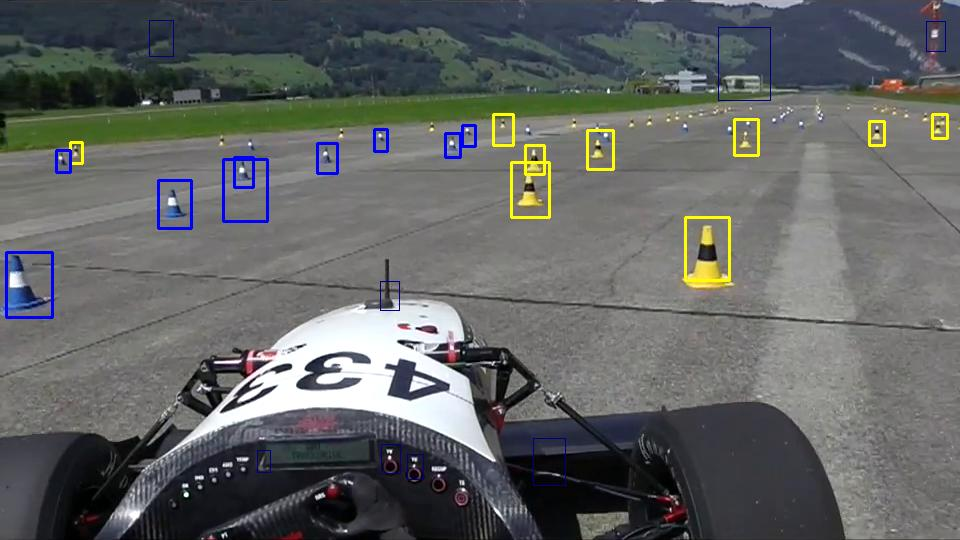
\includegraphics[width=0.45\linewidth]{img/amz/001617}
  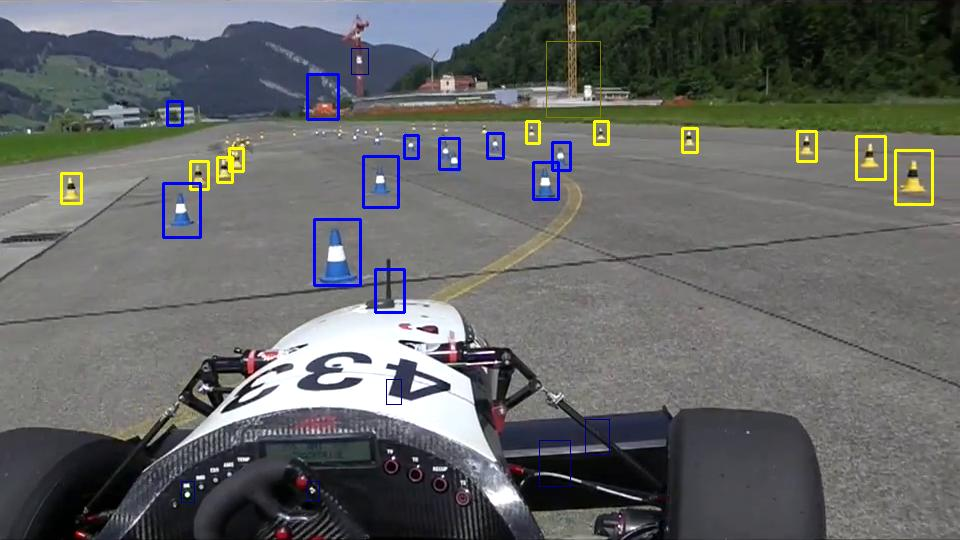
\includegraphics[width=0.45\linewidth]{img/amz/001941}
  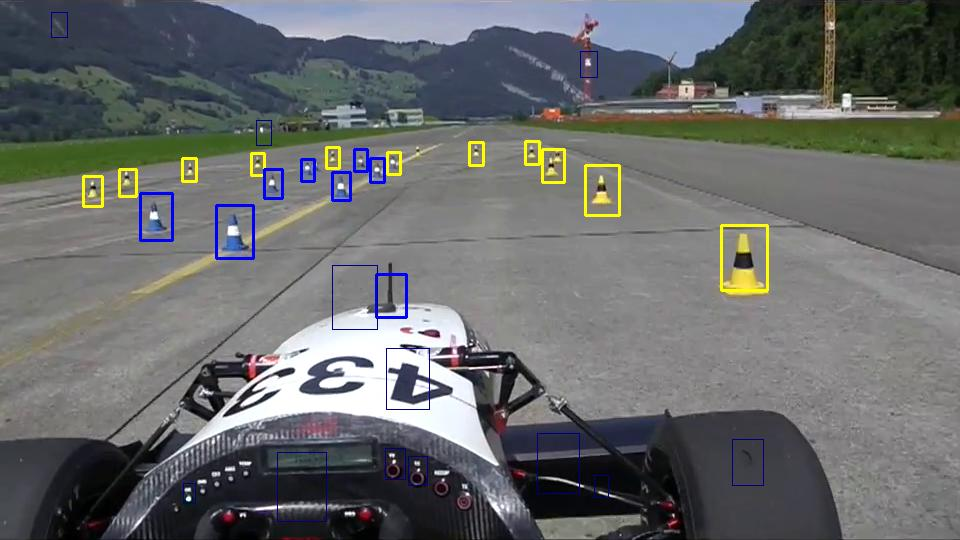
\includegraphics[width=0.45\linewidth]{img/amz/002317}
  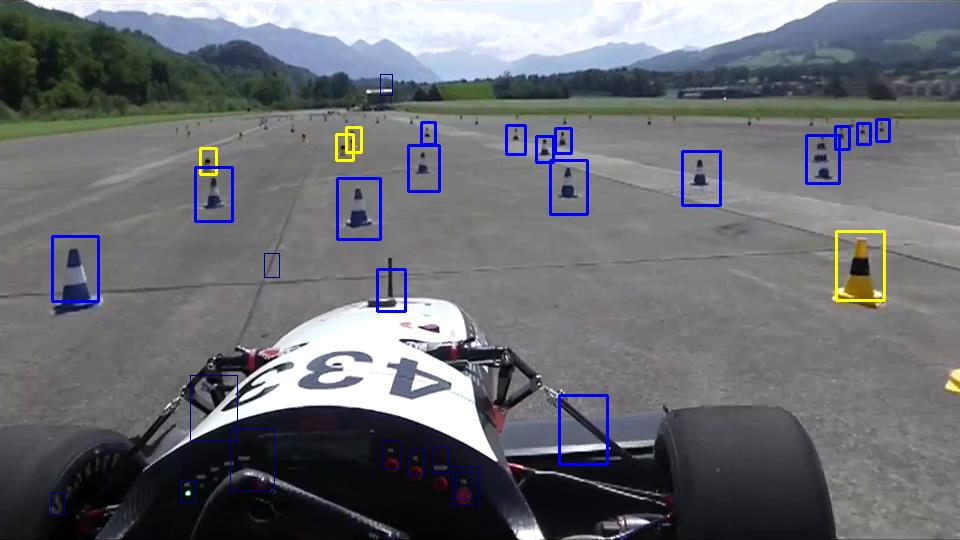
\includegraphics[width=0.45\linewidth]{img/amz/002605}
  \caption{Examples of cone detection. Thick likes indicate firm detections,
    thin lines indicate false detections discarded by the colour
    model. \textsl{Top:} StreetDrone data; \textsl{bottom:} AMZ data.}
  \label{fig:cones}
\end{figure}The filtering and classification of cones by colour is performed as shown
in~\cref{alg:filter}, which estimates for each candidate bounding box produced
by the detector, how well it matches either of the colour models. The example
results of cone detection and localisation are shown in~\cref{fig:cones}.


% The cascade detector consists of different stages. A sliding window is passed through an image, and it is classified by a stage as negative (doesn’t contain the object) or positive (contains the object). If a window is classified as negative, it is rejected and the window slides to the next location. If it is classified as positive, the window is passed to the next stage. The detector will output a detection if the window is classified positive by the final stage.

% RCNN uses selective search to find region proposals in an image. A convolutional neural network is then used to classify each region proposal (about 2000 per image).









% \begin{equation}
%   \label{eq:mahal}
%   d=\sqrt{(\vec{x}-\vec{\mu})\vec{C}^{-1}(\vec{x} - \vec{\mu})'}
% \end{equation}
\section{Localization and Mapping}
Crucial to the situational awareness of the autonomous racing car is the
ability to estimate its state given the observed environment, while at the
same time building up the map of the environment, the paradigm known as
Simultaneous Localization and Mapping (SLAM). This is currently the weakest
part of our project, with more work needed before out SLAM sub-system is
robust enough for FS-AI.

We have investigated a number of SLAM techniques to build a map of the
environment from cone positions: EKF-SLAM~\cite{macsek16},
ORB-SLAM~\cite{artal15}, and LSD-SLAM~\cite{engel14}.
Experimentally, we observed poor reliability with a monocular camera (our
current sensor assumption) and a relatively featureless racing landscape.

\section{Motion Planning}
Assuming the boundaries of the track have been estimated by the SLAM
sub-system, we proceed to discuss the problem of choosing the optimal path for
the vehicle to follow. For a recent review of motion planning techniques for
autonomous vehicles the reader is referred to~\cite{paden16}.

One popular approach to the path planning problem is the discretisation of the
state space such that standard search algorithms like A* and D* can be
used to find the shortest path from the current to the goal state. In the
scenario of autonomous driving the problem with these
algorithms is that they do not consider the non-holonomic nature of the vehicle.
We, therefore, employ an adaptation of A*, termed Hybrid A*~\cite{dolgov08}, which
can deal with the continuous nature of the search space. Hybrid A* was
used effectively for getting a car to navigate and perform complex man\oe{}uvres in urban environments, such as reversing into
parking spots~\cite{petereit12}, and for successfully driving Stanford’s
vehicle ``Junior'' in the DARPA Urban
Challenge~\cite{montemerlo08}. Figure~\cref{fig:comparison} shows the
comparison between A*, D*, and Hybrid A* search strategies.

\paragraph*{Algorithm outline}
Hybrid A* requires spatially discretising the world (track) into $(x, y)$
cells forming a grid (represented as a bitmap, with $0$ representing
traversable space and $1$s the obstacles, \emph{e.g.} track boundaries). This
bitmap is expected to be produced by rasterising the track boundaries
estimated by the SLAM sub-system.  The discretised map which is then used to
close off search space when a cell is expanded by a node, just like standard
A*, but it is possible for multiple nodes lie within an expanded cell.  An
open list $O$ is used to store nodes that have been expanded and might need
further exploration. Once a node is conclusively processed it is placed in the
closed list $C$. Nodes are modeled with coordinates and heading
$(x, y, \theta)$. The starting position and orientation of the car correspond
to the root node. Given a node, a set of new nodes can be calculated from a
pre-defined traveling distance and a set of steering angles, also known as
motion primitives. The number of new nodes to be explored is a tuneable
parameter. The new nodes keep a pointer to their parent node $p$ and are then
added to an open list. The cost $f(n) = g(n)+h(n)$ is computed for each node,
where $g(n)$ is the cost required to reach the node, in our case the distance
travelled, and $h(n)$ is the heuristic which is our estimate of the minimum
cost from the goal. The node with the lowest $f(n)$ is chosen from the open
list and the process from calculating motion primitives is repeated until the
shortest path to the goal is found.

We have experimented with Euclidean and Dubins path length heuristics for
$h(n)$.  Dubins path is the shortest curve that connects two points in
$\mathbb{R}^2$, with the constraints on the curvature of the path, the
tangents of the initial and final points of the path given that the vehicle
that is travelling along the path cannot reverse. (If the vehicle is able to
reverse, then the Reeds-Shepp model can be used.) Dubins path does not does
not take obstacles or barriers into consideration.  Euclidian distance is faster
to calculate, but using it affects the
quality of the produced path (see~\cref{fig:euclidean}).

As with ordinary A*, the open list keeps track of all the nodes that have been
expanded, the node with the lowest $f(n)$ is removed from the list and used
to further calculate the motion primitives.  For performance reasons, we use
the binary min-heap data structure with $O(1)$ time complexity for finding the
minimum $f(n)$ node, $O(\log n)$ for deleting and inserting.  There are
occasions where nodes have the same $f(n)$ we want to perform a tie-break,
this is where we choose the node with the highest $g(n)$ from the two this is
so that it encourages exploration that is closer towards reaching the goal.
\paragraph*{Motion Primitives}

\begin{figure}[t]
  \centering
  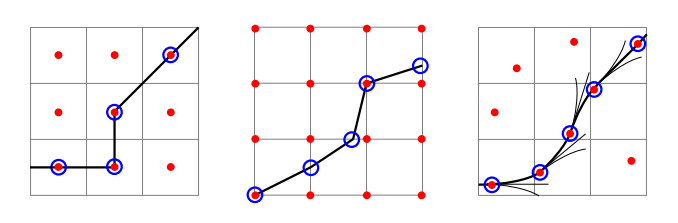
\includegraphics[width=1\linewidth]{img/comparison}
  \vspace{-2em}
  \caption{Comparison of search algorithms. Nodes are represented by the red
    dots. \emph{Left:} A*, \emph{centre:} D*, \emph{right:} hybrid-state
    A*. (From~Dolgov~\emph{et. al}~\cite{dolgov08})}  \vspace{-2em}
  \label{fig:comparison}
\end{figure}
The path is composed of arcs (motion primitives) subject to the following constraints:
\begin{itemize}
\item The distance travelled $d$ has to be enough to exit the cell. For a cell of
  size $s$, it must be the case that $d \ge \sqrt{2}\cdot s$.
  \item The curvature radius $r$ is constrained by the maximum vehicle steering angle $\alpha$.
\end{itemize}
For a vehicle of length $l$ traveling along a motion primitive of length $d$
with a steering angle $\alpha$, the turning angle $\beta = d/(l\tan\alpha)$ and the curvature radius of the turn is $r=d/\beta$. The update to the vehicle state $(x, y, \theta)$ is
calculated as follows:\vspace{-2.5ex}
\begin{align}
  \label{eq:primitive}
  \Delta x = x - r\sin \theta, \qquad x_{\mathrm{new}} &= \Delta x +
             r\sin(\theta+\beta),\\
  \Delta y = y - r\cos \theta, \qquad y_{\mathrm{new}} &= \Delta y +
             r\cos(\theta+\beta),\\
  \theta_{\mathrm{new}} &= \theta + \beta \pmod{2\pi},
\end{align}
The end point of the motion primitive is then used to create a new node
$N = (x_{\mathrm{new}}, y_{\mathrm{new}}, \theta_{\mathrm{new}})$.  Each
motion primitive created is checked for collisions, which involves checking if
any points lie within a specified radius from the front left, front right, and
center point of the vehicle.

We illustrate the operation of the Hybrid A* path planner in~\cref{fig:planning,fig:euclidean}.

\begin{figure}
  \centering
  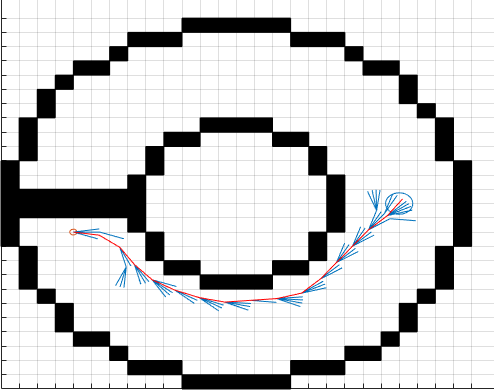
\includegraphics[width=0.49\linewidth]{img/half_cropped}
  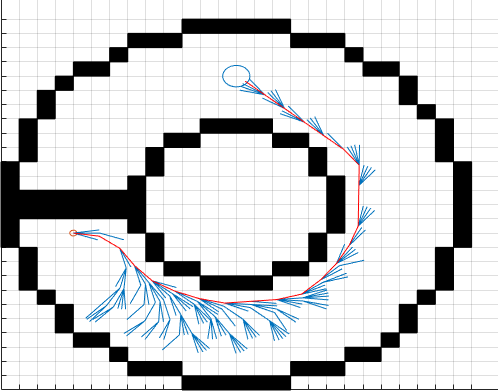
\includegraphics[width=0.49\linewidth]{img/three_quarters_cropped}\\
  % (a)\qquad\qquad\qquad\qquad\qquad\quad(b)\\
  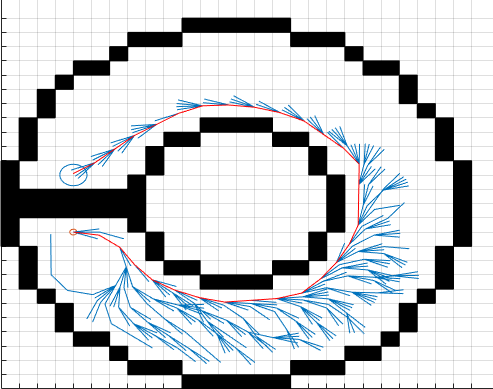
\includegraphics[width=0.49\linewidth]{img/full_cropped}
  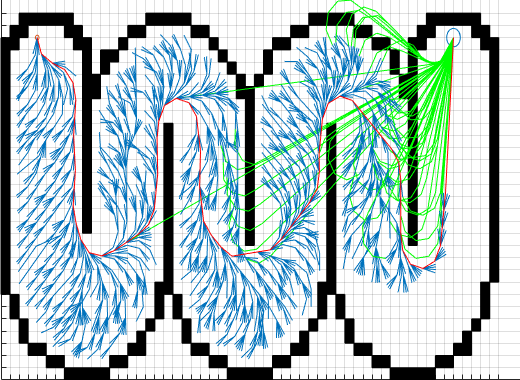
\includegraphics[width=0.49\linewidth]{img/snake_cropped}\\
  % (c)\qquad\qquad\qquad\qquad\qquad\quad(d)\\  
  \raisebox{10ex}{\begin{minipage}{0.49\linewidth}
    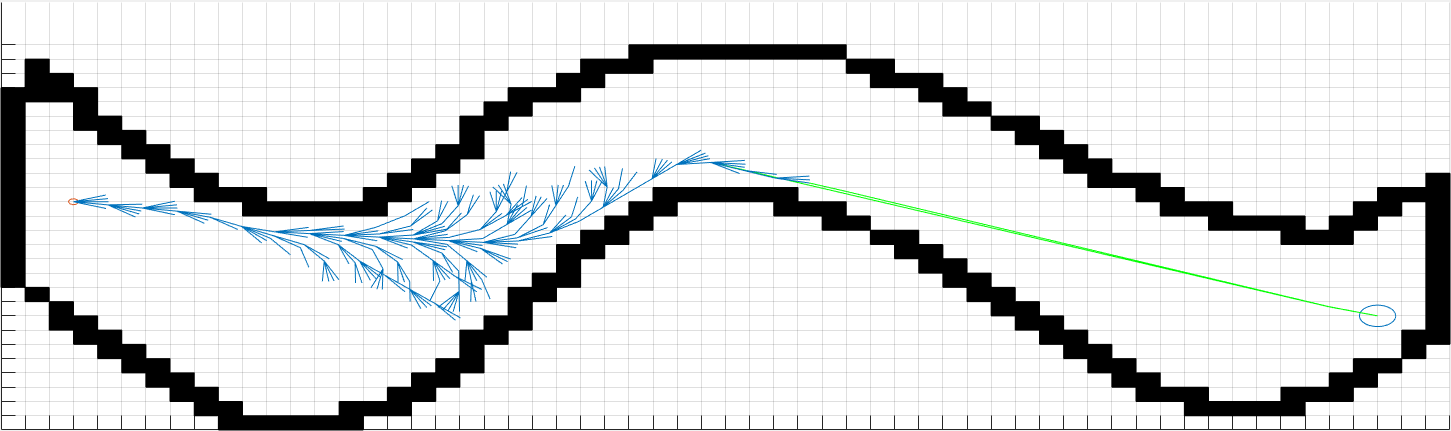
\includegraphics[width=1\linewidth]{img/long_snake_cropped}
    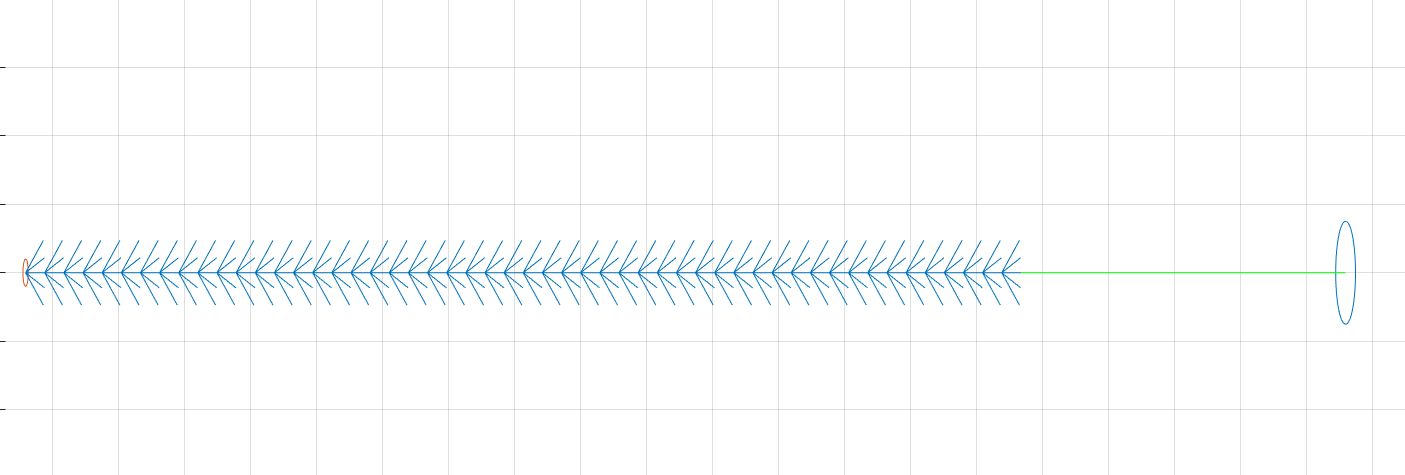
\includegraphics[width=1\linewidth]{img/trivial_cropped}
  \end{minipage}}
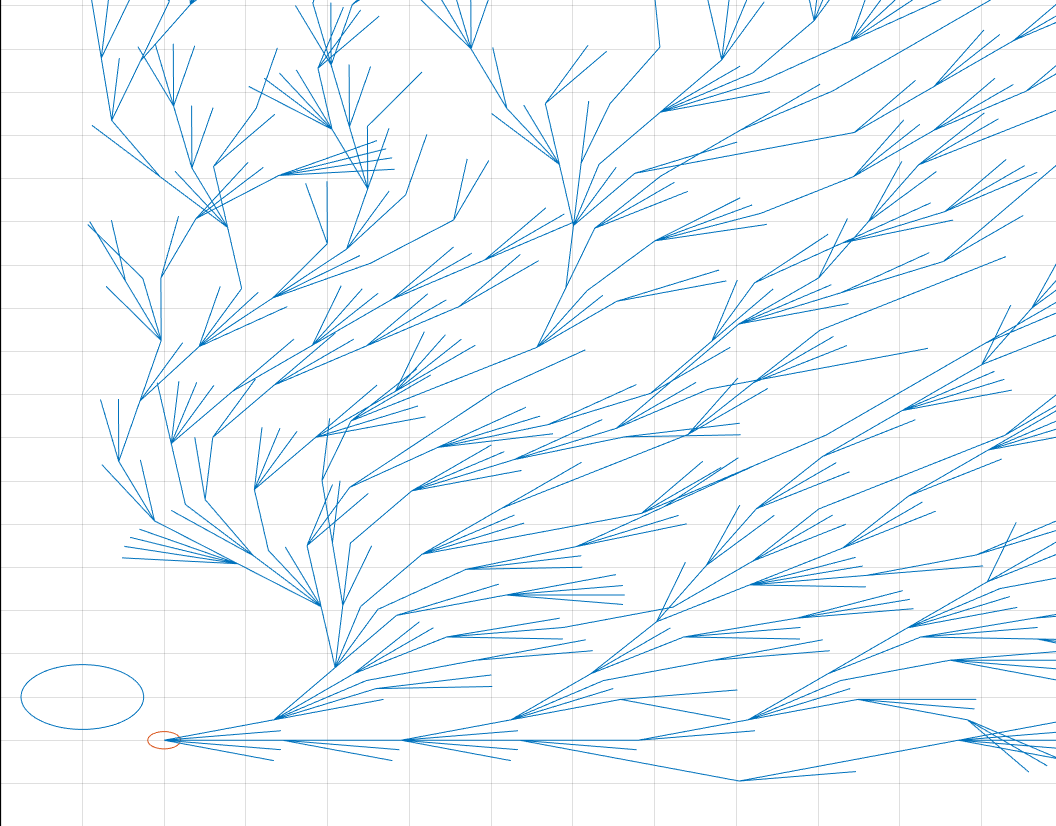
\includegraphics[width=0.49\linewidth]{img/empty_cropped}
% (e)\qquad\qquad\qquad\qquad\qquad\quad(f)\\    
% \label{fig:comparison}
% \end{figure}
% \begin{figure}
%   \centering
  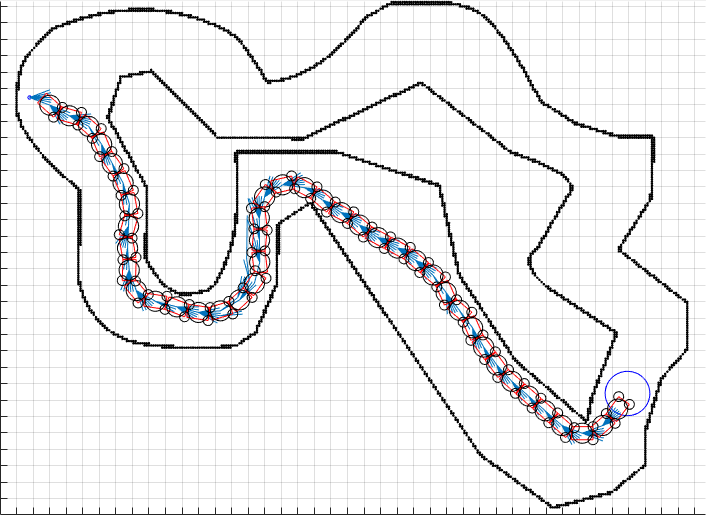
\includegraphics[width=0.49\linewidth]{img/new_collision_astar}
  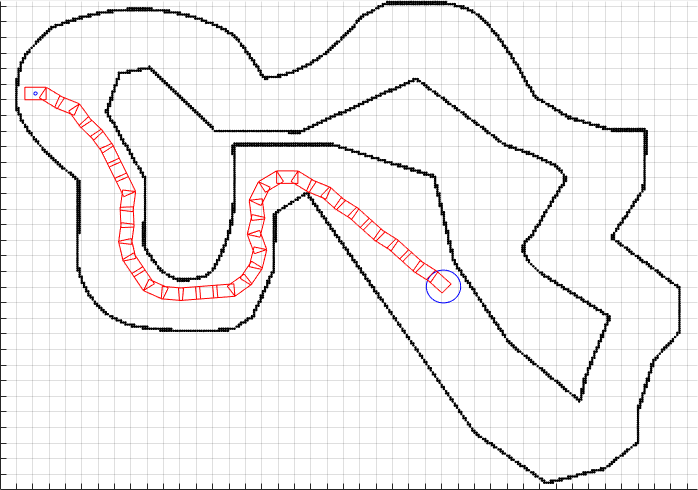
\includegraphics[width=0.49\linewidth]{img/new_solution_skeleton}
  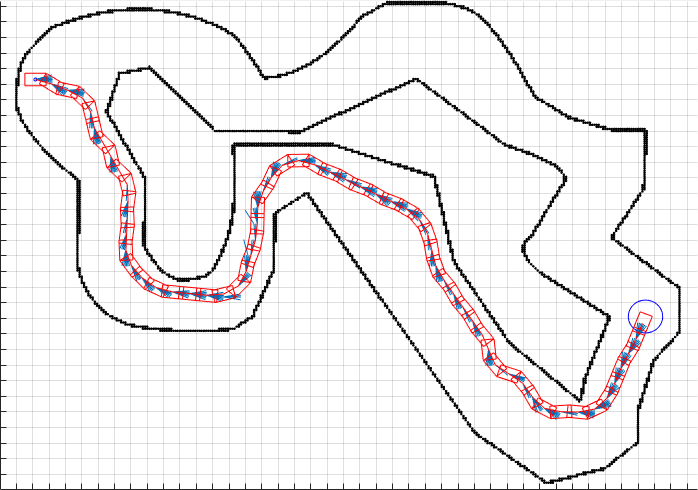
\includegraphics[width=0.49\linewidth]{img/new_long_astar_skeleton}
  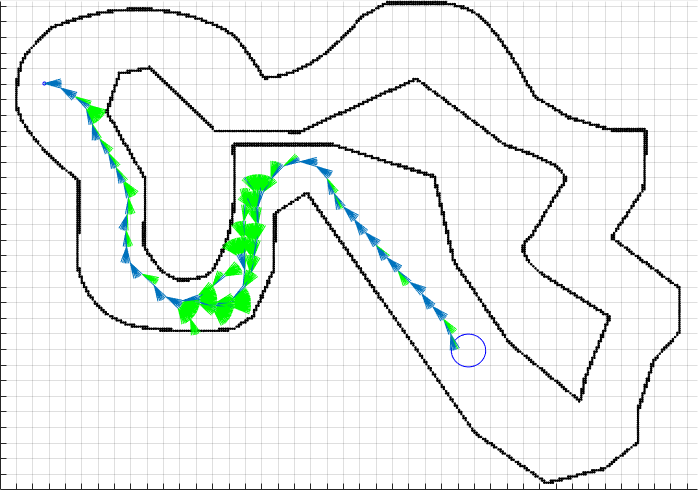
\includegraphics[width=0.49\linewidth]{img/new_astar_fullsearch}\\
  \caption{Illustration of motion planning with Hybrid A* and driveable
    motion primitives.}
\label{fig:planning}
\end{figure}
\begin{figure}
  \centering
  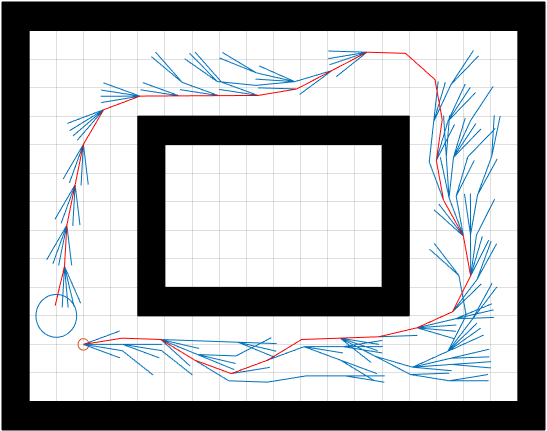
\includegraphics[width=0.49\linewidth]{img/euclidean1_cropped}
  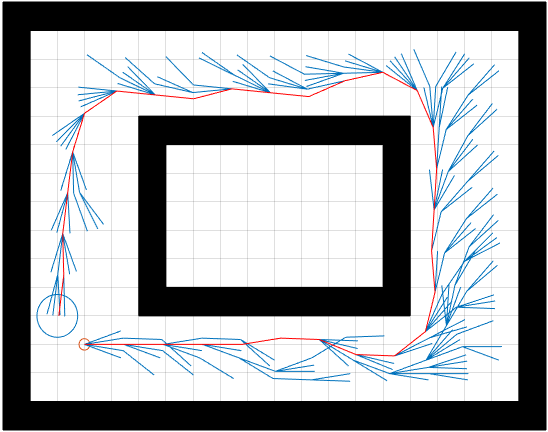
\includegraphics[width=0.49\linewidth]{img/euclidean2_cropped}
  \caption{The effect of introducing additional penalty for large steering
    angles to the Euclidean heuristic.}
  \label{fig:euclidean}
\end{figure}
\begin{figure}
  \centering
  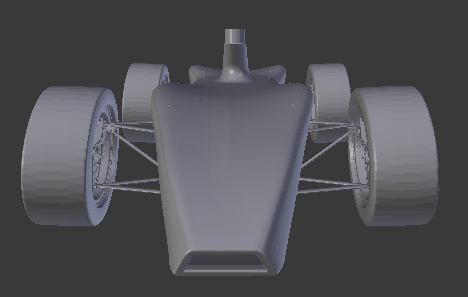
\includegraphics[height=0.18\linewidth]{img/model2}
  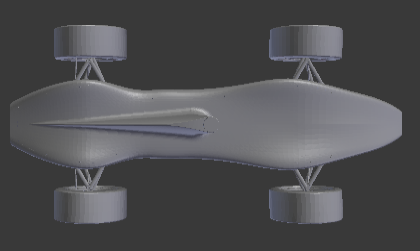
\includegraphics[height=0.18\linewidth]{img/model3}
  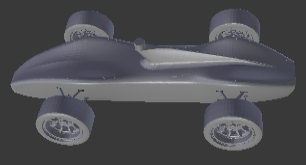
\includegraphics[height=0.18\linewidth]{img/model4}
  \caption{CAD models used in the simulation.}
  \label{fig:cad}
\end{figure}


\paragraph*{Post-optimisation}
Due to the discretization of the steering angle range, it is unlikely for
Hybrid A* to find the global optimum, but the solution is likely to be within
the neighbourhood of it. This typically also leads to producing a path that is
sub-optimal and not smooth, where unnecessary turns are made along the
path. To improve the produced path, this project will aim to post-process the
produced path by performing some local optimization and smoothing.

The path produced by the above Hybrid A*, while close to the optimum, might be
sub-optimal due to discretisation. We employ a further post-optimisation step,
as proposed by Dolgov~\emph{et. al}~\cite{dolgov08}, to improve the length and
smoothness of the path. Let the path be defined by a sequence of vertices
$\vec{x}_i=(x_i, y_i)$, and let $\Delta\vec{x}_i=\vec{x}_i-\vec{x}_{i-1}$. Denote by $\vec{o}_i$ the location of the obstacle
nearest to $\vec{x}_i$ and let $\Delta\phi_i$ be the change in tangential
angle at $\vec{x}_i$. The objective function to be minimised is~\cite{dolgov08}:
\begin{equation}
  \begin{split}
  \mathrm{\min}\leftarrow w_{\rho}\sum_{i=1}^N\rho_d(x_i, y_i)+
  w_o\sum_{i=1}^N(|\vec{x}_i-\vec{o}_i|-d_{\mathrm{max}})^2+\\
  w_{\kappa}\sum_{i=1}^{N-1}\left(\frac{\Delta \phi_i}{|\Delta
      \vec{x}_i|} - \kappa_{\mathrm{max}} \right)^2+
  w_s\sum_{i=1}^{N-1}(\Delta\vec{x}_{i+1}-\Delta\vec{x}_i)^2,
\end{split}
  \label{eq:post}
\end{equation}
where $\rho_d$ is the field of distances to the nearest obstacle,
$\kappa_{\mathrm{max}}$ is the maximum driveable curvature of the path, and
$w_{\rho}$, $w_o$, $w_{\kappa}$, $w_s$ are tuneable weights.
A slightly more sophisticated approach, based on optimisation (in terms of
safety, comfort, efficiency, energy \emph{etc.}) is adopted in~\cite{xu12}.

\section{Simulation}
We have considered several simulation solutions with which to test and tune
our algorithms.

TORCS is used traditionally in racing simulation but difficult to customize and interface with programmatically.
Udacity (based on Unity engine) offers sophisticated graphics but only very
basic mechanical modeling of the vehicle, and no direct simulation of advanced
sensors (e.g. LIDAR). Finally, IPG CarMaker offers extensive realism in
physical simulation, sensor modeling, and affords integration with
MATLAB/Simulink. We have settled on a combination of Udacity with which to
test computer vision parts of the system, and IPG CarMaker for overall system simulation.

\begin{figure}
  \centering
  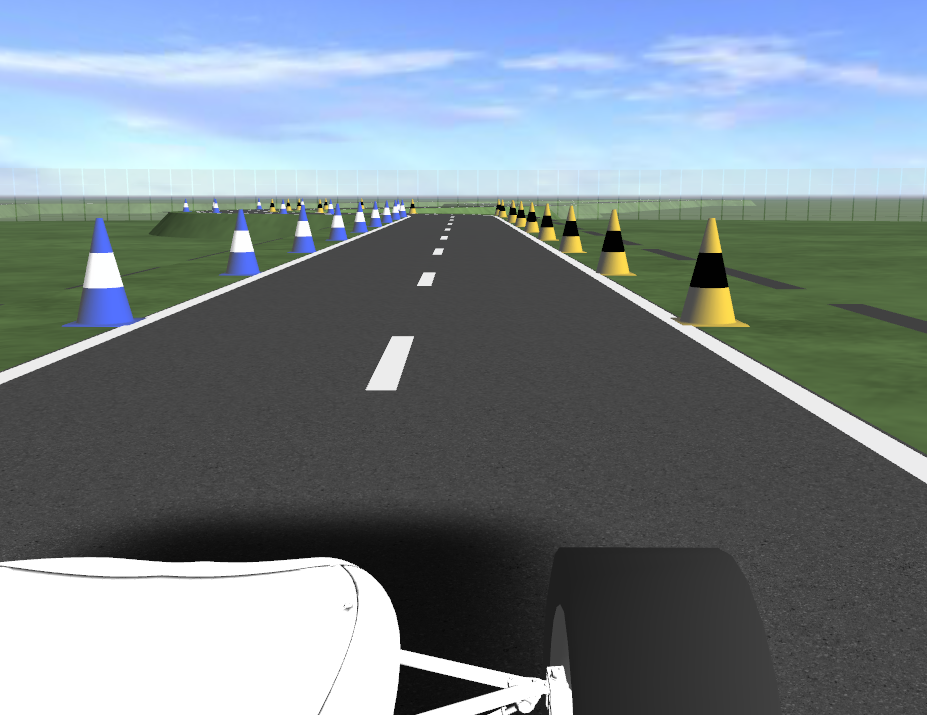
\includegraphics[width=0.45\linewidth]{img/ipg1_cropped}
  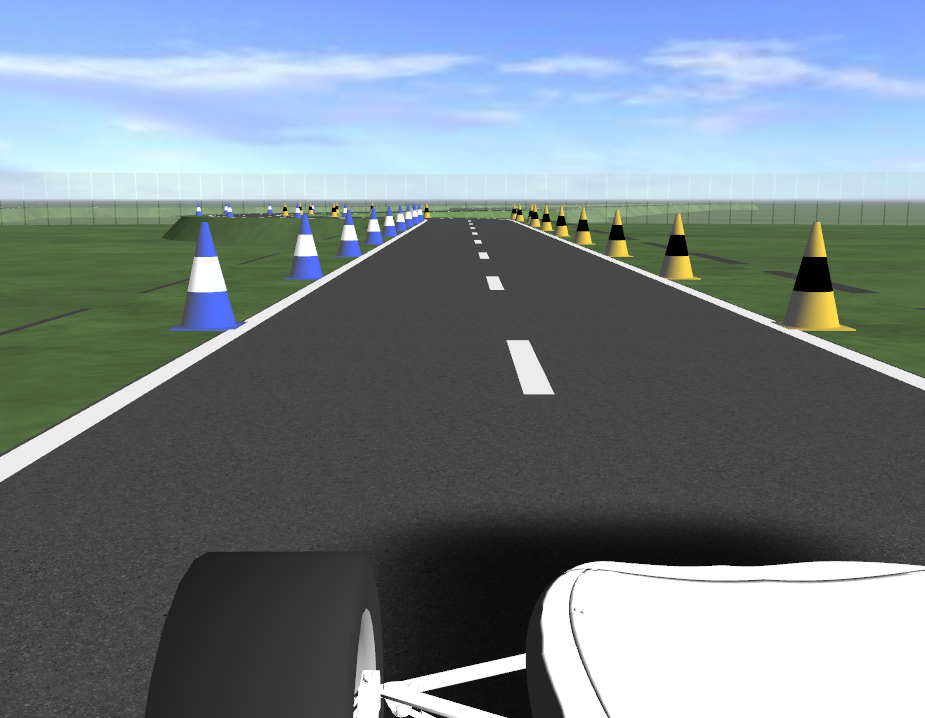
\includegraphics[width=0.45\linewidth]{img/ipg4_cropped}
  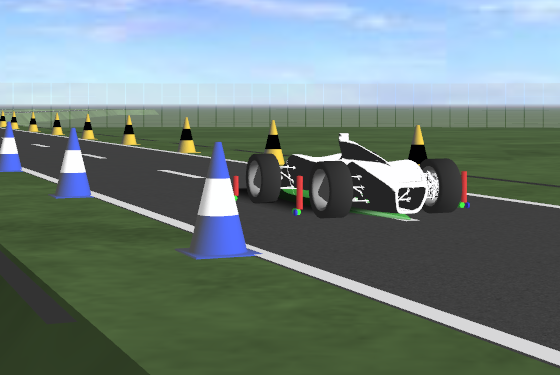
\includegraphics[width=0.45\linewidth]{img/ipg5_cropped}
  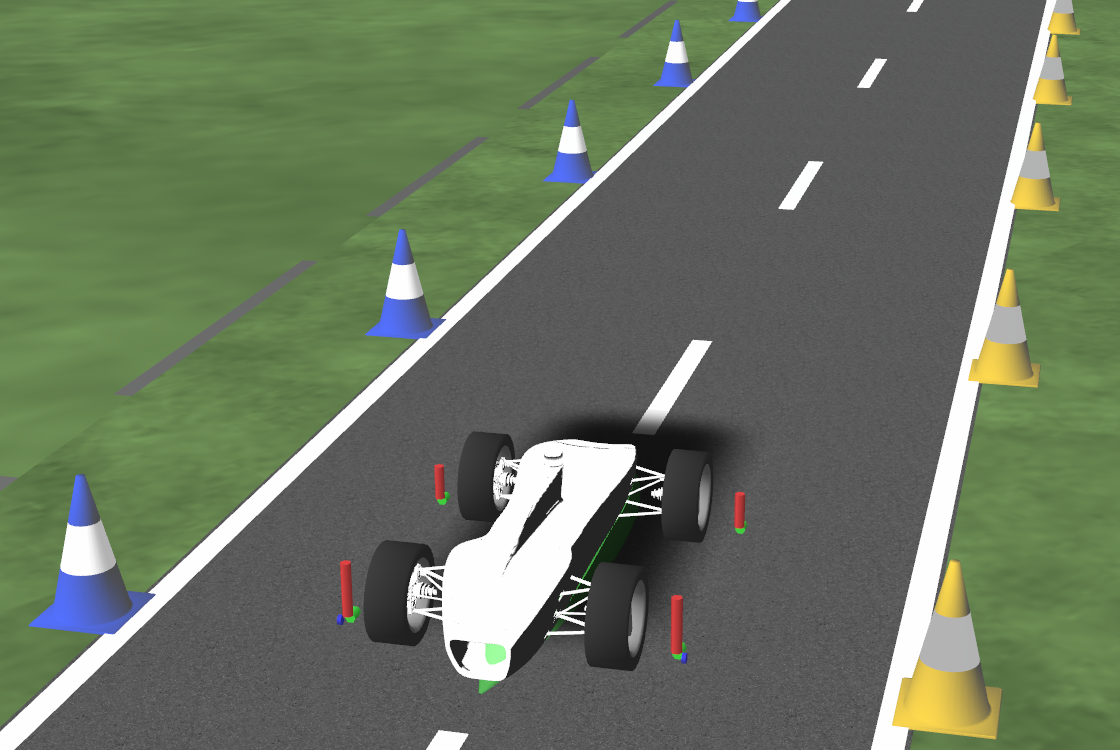
\includegraphics[width=0.45\linewidth]{img/ipg6_cropped}
  \caption{Camera views from the IPG CarMaker simulator.}
  \label{fig:ipg}
\end{figure}
\begin{figure}
  \centering
  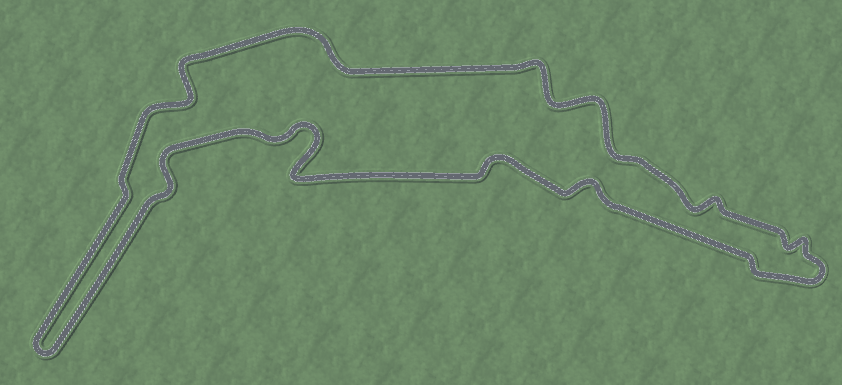
\includegraphics[width=0.7\linewidth]{img/track15_horiz} 
  \caption{Silverstone Formula Student 2015 track modeled in IPG.}
  \label{fig:silverstone}
    \vspace{-2em}
\end{figure}

\begin{table*}
  \caption{Vehicle parameters in IPG CarMaker. In bold: measured from the
    platform vehicle, other parameters are estimated.}
  \centering
  \begin{tabular}{llllll}
    \toprule
    Parameter & Value & Parameter & Value & Parameter & Value\\
    \midrule
    Length & \textbf{1.170 m} & Height & \textbf{0.229 m} & Body mass &
                                                                        \textbf{191.84 kg}\\
    Overall mass & \textbf{308.90 kg} & Rotation (torsion) & 5000 Nm/deg & Rotation (bending) & 15000 Nm/deg\\
    Front wheel carrier mass & 1.67 kg & Back wheel carrier mass & 1.44 kg &
                                                                           Wheel
                                                                           mass
                                                      & 8.71 kg\\
    Engine mount stiffness & 50000 N/m & Engine mount damping & 500 Ns/m &
                                                                           Suspension
                                                                           spring
                                                                           stiffness
                                                      & 35000 N/m\\
    Front damping (push) & 2500 Ns/m & Front damping (pull) & 5000 Ns/m & Buffer
                                                                        stiffness
                                                                        (push)
                                                      & 5000 N/m\\
    Buffer stiffness (pull) & 5000 N/m & Front stabilizer stiffness & 287 N/m &
                                                                              Rear
                                                                                stabilizer
                                                                                stiffness
                                                      & 191.9 N/m\\




                      Steering pinion angle & 100 rad/m & Motor power & 17 kW &
                                                                               Motor torque & 55 Nm\\
    Aerodynamic reference area & 2 m$^2$ & Aerodynamic reference length & 1.3 m
                                          & &\\
        \bottomrule
  \end{tabular}
  \label{tab:ipg}
\end{table*}

We have modeled the platform vehicle from FSUK 2018 competition in IPG
CarMaker (see~\cref{fig:cad,fig:ipg}), as well as mocked up a number of test scenarios,
\emph{e.g.} the Silverstone circuit (see~\cref{fig:silverstone}). Some of the vehicle
parameters we are using are summarised in~\cref{tab:ipg}. We are employing IPG
CarMaker's integration with MATLAB/Simulink to run the tests programmatically.

Work is currently underway to improve the realism of simulation, both
graphically and mechanically, to bring it closer to the conditions of the FSUK
competition. We intend to make our models and APIs publicly available, so that
all teams can take advantage of a common, convenient, and powerful testbed.


\section{Future Work}
Currently, the weakest part of the project is the SLAM sub-system, which we
intend to finish in time for the 2019 competition.

A number of improvements will concern trajectory planning. At
present, the trajectories are planned with no regard for velocity
profiles. For optimal racing performance, it is necessary that the trajectory
and the velocity be optimised jointly.  This is a challenging problem, and the
approach we are currently implementing involves iterative optimisation of
both, and is due to~\cite{xu12}.

As far as the sensors are concerned, we have so far concentrated only on the
hardest scenario, whereby the vehicle is equipped only with a monocular
camera. Future work will include techniques for cone detection from LIDAR
data, a stereopair of cameras, and fusion of these.

Further, given the stellar success of deep reinforcement learning, in some challenging
tasks achieving better than human performance~\cite{mnih15}, we intend to
investigate (in a simulated environment) whether reinforcement learning can be
applied to driverless racing control, and compare it with traditional control
techniques.
We further intend to compare the performance of the existing control
sub-systems (including the one based on reinforcement learning) with that of a
human driver, and explore whether any heuristics, derived from observing
human control, can be employed to improve automatic control.

A path following controller (\emph{e.g.}~\cite{ni17}) remains to be implemented. Optimal tuning of path following
controller will involve accurate modeling of drive-by-wire controls, such as
throttle, steering, and braking-by-wire.

Finally, integration of all components into a complete system presents a
non-trivial task. We are currently transitioning to using the Robot
Operating System (ROS) as a platform for system integration, modularisation,
and communication.

\section*{Acknowledgements}
The authors would like to thank MathWorks for providing competition MATLAB
licenses and IPG Automotive for providing the IPG CarMaker simulator.
\bibliographystyle{IEEEtran}
\bibliography{adr}
% \input{./bibs/amz_icra01_arxiv.bbl}

\begin{acronym}
\acro{SLAM}{Simultaneous Localization and Mapping}
\acro{ECU}{Electronic Control Unit}
\end{acronym}

\end{document}


%  LocalWords:  ieeetrantools
